%%%%%%%%%%%%%%%%%%%%%%%%%%%%%%%%%%%%%%%%%%%%%%
% Header
\documentclass[12pt]{article}
\usepackage[english]{babel}
\usepackage[utf8x]{inputenc}
\usepackage{hyperref}
\usepackage{graphicx}
\usepackage{fullpage}
\usepackage[lastexercise]{exercise}
\usepackage{enumitem}
\graphicspath{{./weekly_content/img/}}

\setlength{\parindent}{0cm}

\renewcommand{\ExerciseHeader}{\large\textbf{\ExerciseName~\ExerciseHeaderNB} - \textbf{\ExerciseTitle}\medskip}

\renewcommand{\ExePartHeader}{\medskip\textbf{\ExePartName\ExePartHeaderNB\ExePartHeaderTitle\medskip}}

\begin{document}
%%%%%%%%%%%%%%%%%%%%%%%%%%%%%%%%%%%%%%%%%%%%%%
\title{Exercises -- Week 1: Introduction to Python}
\subsubsection*{EMAT10007 -- Introduction to Computer Programming}
\subsection*{\Large Exercises -- Week 1. \\ Objects, Variables and Operators}

\noindent\fbox{%
    \parbox{\textwidth}{%
        \subsection*{Getting Started: How to open software}
        \subsubsection*{PyCharm IDE (Integrated Development Environment)}
        \begin{itemize}
            \item{Open PyCharm on a Linux lab computer}
            \begin{itemize}
                \item{Click on Activities in the top left corner of the screen.}
                \item{Open 'Terminal' from the menu tab.}
            \end{itemize}
            \item{To instead install PyCharm on your personal computer}
            \begin{itemize}
                \item{Click on Activities in the top left corner of the screen.}
                \item{Open 'Terminal' from the menu tab.}
                \item{Type or copy and paste the following:}
    	    \item{Press enter}
            \end{itemize}
        \end{itemize}
        \subsubsection*{Online code editors}
        \begin{itemize}
            \item{Open 'Terminal' from the menu tab.}
            \item{Type or copy and paste the following:}
        \end{itemize}
    }        
}%

\vspace{15}

\noindent\fbox{%
    \parbox{\textwidth}{%
        \subsection*{Getting Started: How to save your work}
        \subsubsection*{PyCharm IDE}
        \begin{itemize}
            \item{Open 'Terminal' from the menu tab.}
        \end{itemize}
        \subsubsection*{Online code editors}
        \begin{itemize}
            \item{Open 'Terminal' from the menu tab.}
        \end{itemize}
    }        
}%

\vspace{15}

\noindent\fbox{%
    \parbox{\textwidth}{%
        \subsection*{Rules for naming variables}
	\begin{itemize}
            \item Variable names may contain letters or numbers
            \item Variable names must begin with a letter
            \item Variable names are case sensitive ({\tt time} is not the same as {\tt Time})		
            \item Some {\tt keywords} are reserved by the Python language and cannot be used as variable names. For a full list of keywords reserved by Python, enter the following run the following comand in the editor you are using:
            
    		\vspace{0.5em}
    		{\tt help("keywords")}
    		\vspace{0.5em}
    		
    	\item{Use a consistent naming convention:
            \begin{itemize}
                \item {\tt snake\_case}: lower case letters, words separated by underscore ({\tt \_})
                \item {\tt camel\_Case}: first letter of each word capitalised, excluding first word
                \item {\tt Pascal\_Case}: first letter of each word capitalised
            \end{itemize}
            }
    \end{itemize}
    }        
}%



\begin{Exercise}[title=Objects and Variables]  \label{Ex:Numbers}
% \ExeText{Python can be used as a calculator. You can input operations, and store the results of operations as variables for use in additional calculations.}
    \Question{Create two variables, a and b and assign an integer value to each variable. Calculate the product of a and b and print the result.}
    \Question{Create two variables, c and d and assign a floating point value to each variable. Calculate the difference between c and d and store the result as a new variable, e. Print e.}
    \Question{Overwrite the value of the new variable you just created with the value $\frac{a+b}{3}$.
    \Question{Find the remainder when c is divided by d and print the result.}.
        \Question{Cast c as an integer}
        \Question{Cast b as a string}
        \Question{Cast a as a Boolean}
        \Question{Create a new variable, f and assign a string value to it}
        \Question{Print the last character in the string assigned to f}
        \Question{Create two variables, g and h and assign a string value to each variable. Connect the two strings using the addition (+) operator. Can you work out how to separate the two strings with a space when connecting them? }.
    \end{Exercise}

\begin{Exercise}[title=Arithmetic Operators] \label{Ex:Strings}
    \Question{Write a program that finds the volume ($V$) of a sphere with diameter 30cm, then displays the value with the correct units.\\ Volume of a sphere: $$V = \frac{4}{3}\pi r^2$$  \\ $r = $ radius. Assume $\pi = $ 3.142}
    \Question{Find the Euclidean distance, $d$ between two points with 3-dimensional position vectors ${\mathbf{a} = [5.0, 4.5, 2.0]$ and ${\mathbf{b} = [10.6, 11.5, 6.2]$ using $$d = \sqrt{(x_a - x_b)^2 + (y_a - y_b)^2 + (z_a - z_b)^2}$$}
    % \Question{Modular arithmetic is a system for integers, where numbers "wrap around" when reaching a certain value called the modulus. For example, for example adding 4 hours to 9 o'clock gives 1 o'clock. \\ Consider the hours on a clock. The modulus ($mod$) is the number of hours = 12. The minimum value ($min$) is 1. The new time $t_1$, given the current time, $t_0$, and the number of hours shifted $n$ can be found by: $$t_1 = (t_0 - min + (n \% mod) + n ) \% n + min$$. Use this expression }
\end{Exercise}

\begin{Exercise}[title=Comparison Operators]  

\ExeText{Create three variables x=1.2, y=3.3 and z = 4.0.}
    \Question{Write an expression to test if x is greater than or equal to y}
    \Question{Write an expression to test if x multiplied by 3 is less than y}
    \Question{Write an expression to test if x is less than y, and y is less than z}
    \Question{Write an expression to test if y is less than both x and z}
    \Question{Write an expression to test if the sum of x and 2.1 is equal to y}
\ExeText{Change the values of x, y and z to verify that the expressions you have written still work}
\end{Exercise}

\begin{Exercise}[title=Logical Operators] 

\ExeText{Create four variables u=2, v=-4, w = 1 and x=5}
    \Question{Write an expression to test if u is greater than v and w is less than x}
    \Question{Write an expression to test if v, w and x are all smaller than u}
    \Question{Write an expression to test if at least one of  v, w and x are greater than u.}
    \Question{Write an expression to test if x divided by 2 is less than or equal to u - 1.2}
    \Question{Write an expression to test if the value of any of the variables are negative}
\ExeText{Change the values of u, v, w, and x to verify that the expressions you have written still work}
\end{Exercise}	

\begin{Exercise}[title=Putting it all together]
\begin{figure}[!h]
    \centering
    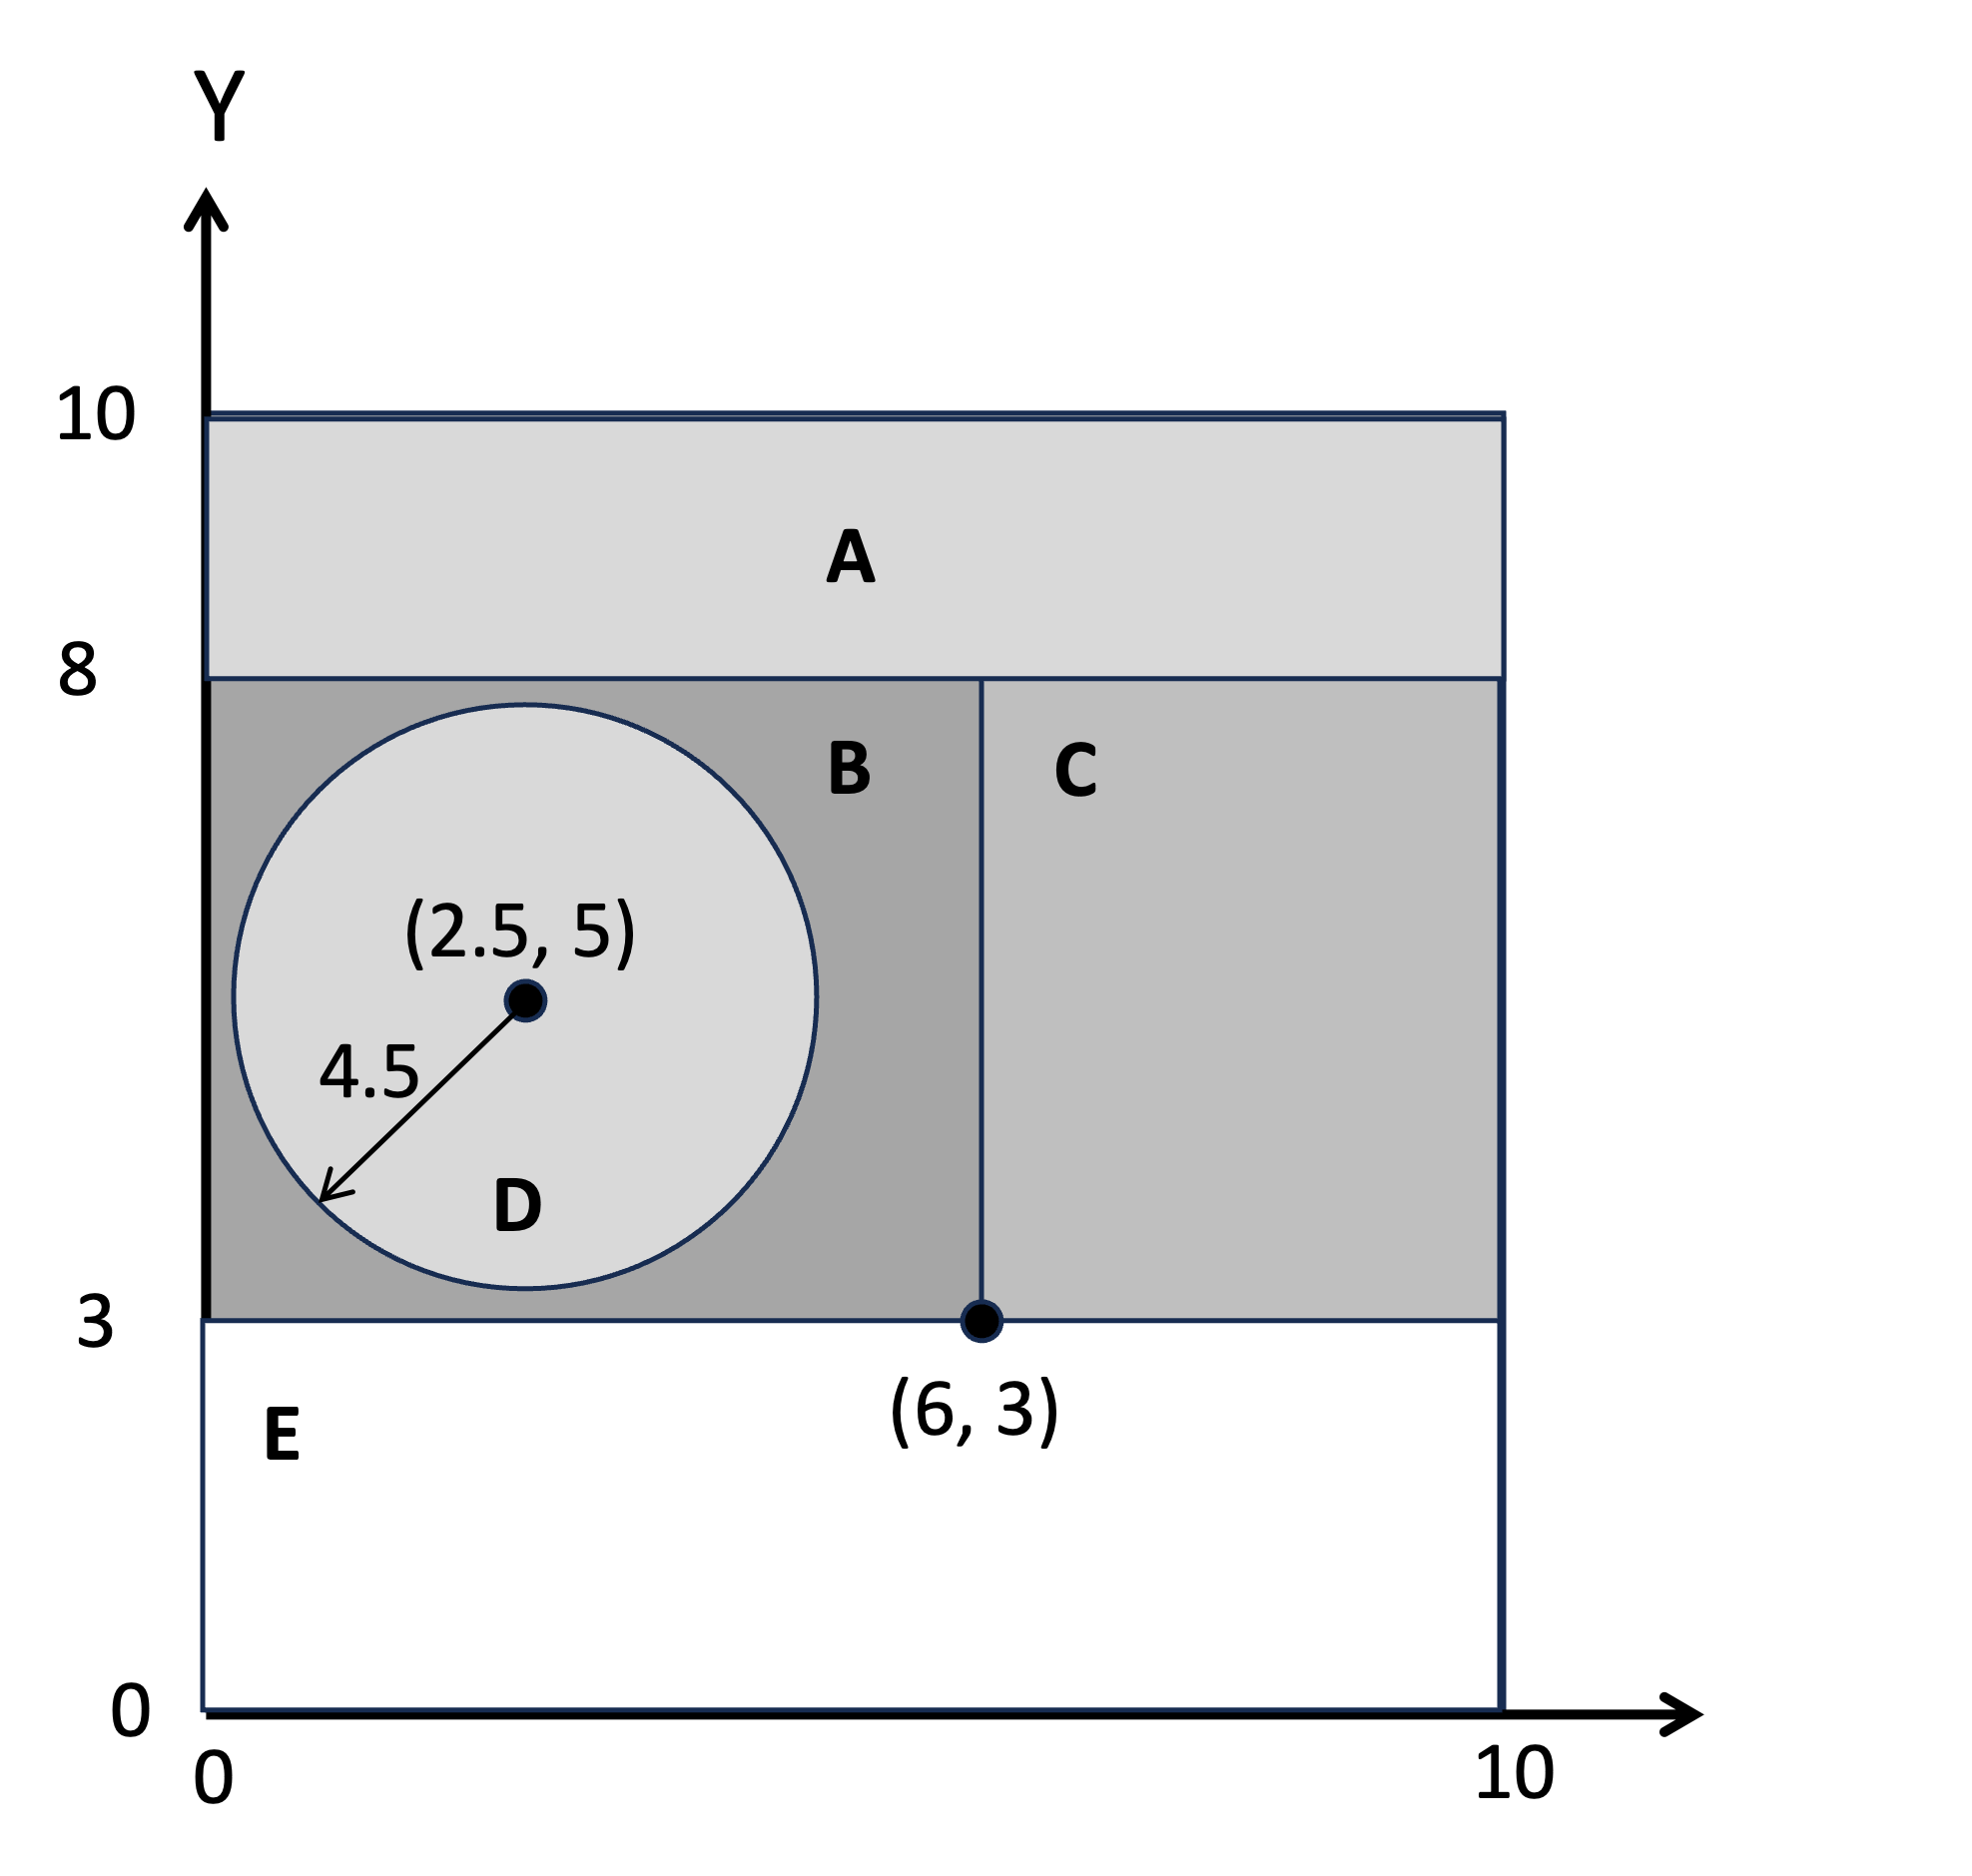
\includegraphics[height=7.5cm]{region}
    \caption{Map}
    \label{fig:map}
\end{figure}

\ExeText{A point lies on a map (Figure \ref{fig:map}). Each region excludes its outer boundary. For a given point (x,y) where x and y are each a floating point number in the range (0, 10)}
    \Question{Write an expression to test if the point is in region A}
    \Question{Write an expression to test if the point is in region B}
    \Question{Write an expression to test if the point is in region C}
    \Question{Write an expression to test if the point is in region D}
    \Question{Write an expression to test if the point is in region E}
    \Question{Combine these statements in a different order to minimise the number of times you need to code each comparison explicitly.}
\end{Exercise}





\end{document}